% Options for packages loaded elsewhere
% Options for packages loaded elsewhere
\PassOptionsToPackage{unicode}{hyperref}
\PassOptionsToPackage{hyphens}{url}
\PassOptionsToPackage{dvipsnames,svgnames,x11names}{xcolor}
%
\documentclass[
  russian,
]{article}
\usepackage{xcolor}
\usepackage[top=20mm,left=20mm,right=20mm,bottom=20mm]{geometry}
\usepackage{amsmath,amssymb}
\setcounter{secnumdepth}{5}
\usepackage{iftex}
\ifPDFTeX
  \usepackage[T1]{fontenc}
  \usepackage[utf8]{inputenc}
  \usepackage{textcomp} % provide euro and other symbols
\else % if luatex or xetex
  \usepackage{unicode-math} % this also loads fontspec
  \defaultfontfeatures{Scale=MatchLowercase}
  \defaultfontfeatures[\rmfamily]{Ligatures=TeX,Scale=1}
\fi
\usepackage{lmodern}
\ifPDFTeX\else
  % xetex/luatex font selection
  \setmainfont[]{Times New Roman}
  \setsansfont[]{Arial}
  \setmonofont[]{Courier New}
\fi
% Use upquote if available, for straight quotes in verbatim environments
\IfFileExists{upquote.sty}{\usepackage{upquote}}{}
\IfFileExists{microtype.sty}{% use microtype if available
  \usepackage[]{microtype}
  \UseMicrotypeSet[protrusion]{basicmath} % disable protrusion for tt fonts
}{}
\makeatletter
\@ifundefined{KOMAClassName}{% if non-KOMA class
  \IfFileExists{parskip.sty}{%
    \usepackage{parskip}
  }{% else
    \setlength{\parindent}{0pt}
    \setlength{\parskip}{6pt plus 2pt minus 1pt}}
}{% if KOMA class
  \KOMAoptions{parskip=half}}
\makeatother
% Make \paragraph and \subparagraph free-standing
\makeatletter
\ifx\paragraph\undefined\else
  \let\oldparagraph\paragraph
  \renewcommand{\paragraph}{
    \@ifstar
      \xxxParagraphStar
      \xxxParagraphNoStar
  }
  \newcommand{\xxxParagraphStar}[1]{\oldparagraph*{#1}\mbox{}}
  \newcommand{\xxxParagraphNoStar}[1]{\oldparagraph{#1}\mbox{}}
\fi
\ifx\subparagraph\undefined\else
  \let\oldsubparagraph\subparagraph
  \renewcommand{\subparagraph}{
    \@ifstar
      \xxxSubParagraphStar
      \xxxSubParagraphNoStar
  }
  \newcommand{\xxxSubParagraphStar}[1]{\oldsubparagraph*{#1}\mbox{}}
  \newcommand{\xxxSubParagraphNoStar}[1]{\oldsubparagraph{#1}\mbox{}}
\fi
\makeatother


\usepackage{longtable,booktabs,array}
\newcounter{none} % for unnumbered tables
\usepackage{calc} % for calculating minipage widths
% Correct order of tables after \paragraph or \subparagraph
\usepackage{etoolbox}
\makeatletter
\patchcmd\longtable{\par}{\if@noskipsec\mbox{}\fi\par}{}{}
\makeatother
% Allow footnotes in longtable head/foot
\IfFileExists{footnotehyper.sty}{\usepackage{footnotehyper}}{\usepackage{footnote}}
\makesavenoteenv{longtable}
\usepackage{graphicx}
\makeatletter
\newsavebox\pandoc@box
\newcommand*\pandocbounded[1]{% scales image to fit in text height/width
  \sbox\pandoc@box{#1}%
  \Gscale@div\@tempa{\textheight}{\dimexpr\ht\pandoc@box+\dp\pandoc@box\relax}%
  \Gscale@div\@tempb{\linewidth}{\wd\pandoc@box}%
  \ifdim\@tempb\p@<\@tempa\p@\let\@tempa\@tempb\fi% select the smaller of both
  \ifdim\@tempa\p@<\p@\scalebox{\@tempa}{\usebox\pandoc@box}%
  \else\usebox{\pandoc@box}%
  \fi%
}
% Set default figure placement to htbp
\def\fps@figure{htbp}
\makeatother



\ifLuaTeX
\usepackage[bidi=basic,shorthands=off,provide=*]{babel}
\else
\usepackage[bidi=default,shorthands=off,provide=*]{babel}
\fi
\ifPDFTeX
\else
\babelfont{rm}[]{Times New Roman}
\fi
\ifLuaTeX
  \usepackage{selnolig} % disable illegal ligatures
\fi


\setlength{\emergencystretch}{3em} % prevent overfull lines

\providecommand{\tightlist}{%
  \setlength{\itemsep}{0pt}\setlength{\parskip}{0pt}}



 


\makeatletter
\@ifpackageloaded{tcolorbox}{}{\usepackage[skins,breakable]{tcolorbox}}
\@ifpackageloaded{fontawesome5}{}{\usepackage{fontawesome5}}
\definecolor{quarto-callout-color}{HTML}{909090}
\definecolor{quarto-callout-note-color}{HTML}{0758E5}
\definecolor{quarto-callout-important-color}{HTML}{CC1914}
\definecolor{quarto-callout-warning-color}{HTML}{EB9113}
\definecolor{quarto-callout-tip-color}{HTML}{00A047}
\definecolor{quarto-callout-caution-color}{HTML}{FC5300}
\definecolor{quarto-callout-color-frame}{HTML}{acacac}
\definecolor{quarto-callout-note-color-frame}{HTML}{4582ec}
\definecolor{quarto-callout-important-color-frame}{HTML}{d9534f}
\definecolor{quarto-callout-warning-color-frame}{HTML}{f0ad4e}
\definecolor{quarto-callout-tip-color-frame}{HTML}{02b875}
\definecolor{quarto-callout-caution-color-frame}{HTML}{fd7e14}
\makeatother
\makeatletter
\@ifpackageloaded{caption}{}{\usepackage{caption}}
\AtBeginDocument{%
\ifdefined\contentsname
  \renewcommand*\contentsname{Содержание}
\else
  \newcommand\contentsname{Содержание}
\fi
\ifdefined\listfigurename
  \renewcommand*\listfigurename{Список Иллюстраций}
\else
  \newcommand\listfigurename{Список Иллюстраций}
\fi
\ifdefined\listtablename
  \renewcommand*\listtablename{Список Таблиц}
\else
  \newcommand\listtablename{Список Таблиц}
\fi
\ifdefined\figurename
  \renewcommand*\figurename{Рисунок}
\else
  \newcommand\figurename{Рисунок}
\fi
\ifdefined\tablename
  \renewcommand*\tablename{Таблица}
\else
  \newcommand\tablename{Таблица}
\fi
}
\@ifpackageloaded{float}{}{\usepackage{float}}
\floatstyle{ruled}
\@ifundefined{c@chapter}{\newfloat{codelisting}{h}{lop}}{\newfloat{codelisting}{h}{lop}[chapter]}
\floatname{codelisting}{Список}
\newcommand*\listoflistings{\listof{codelisting}{Список Каталогов}}
\makeatother
\makeatletter
\makeatother
\makeatletter
\@ifpackageloaded{caption}{}{\usepackage{caption}}
\@ifpackageloaded{subcaption}{}{\usepackage{subcaption}}
\makeatother
\usepackage{bookmark}
\IfFileExists{xurl.sty}{\usepackage{xurl}}{} % add URL line breaks if available
\urlstyle{same}
\hypersetup{
  pdftitle={Задачи по Эконометрике-2: logit/probit-модель},
  pdfauthor={Н.В. Артамонов, А. Н. Лата (МГИМО МИД России)},
  pdflang={ru},
  colorlinks=true,
  linkcolor={blue},
  filecolor={Maroon},
  citecolor={Blue},
  urlcolor={Blue},
  pdfcreator={LaTeX via pandoc}}


\title{Задачи по Эконометрике-2: logit/probit-модель}
\author{Н.В. Артамонов, А. Н. Лата (МГИМО МИД России)}
\date{}
\begin{document}
\maketitle

\renewcommand*\contentsname{Содержание}
{
\setcounter{tocdepth}{3}
\tableofcontents
}

\section{Нормальное и логистическое
распределения}\label{ux43dux43eux440ux43cux430ux43bux44cux43dux43eux435-ux438-ux43bux43eux433ux438ux441ux442ux438ux447ux435ux441ux43aux43eux435-ux440ux430ux441ux43fux440ux435ux434ux435ux43bux435ux43dux438ux44f}

\textbf{Стандартное нормальное (гауссово) распределение \(N(0, 1)\)}

\begin{itemize}
\item
  Плотность вероятности:
  \[\phi(t) = \frac{1}{\sqrt{2\pi}} \exp\left(-\frac{t^2}{2}\right), \quad t \in \mathbb{R}\]
\item
  (Кумулятивная) функция распределения:
  \[\Phi(x) = \int\limits_{-\infty}^x \phi(t) \, dt, \quad x \in \mathbb{R}\]
\end{itemize}

\begin{center}\rule{0.5\linewidth}{0.5pt}\end{center}

\textbf{Логистическое распределение}

\begin{itemize}
\item
  (Кумулятивная) функция распределения:
  \[\Lambda(x) = \frac{\exp(x)}{1 + \exp(x)}, \quad x \in \mathbb{R}\]
\item
  Плотность вероятности:
  \[\lambda(x) = \Lambda'(x) = \frac{\exp(x)}{(1 + \exp(x))^2}, \quad x \in \mathbb{R}\]
\end{itemize}

\begin{center}\rule{0.5\linewidth}{0.5pt}\end{center}

Плотности на одном графике

\pandocbounded{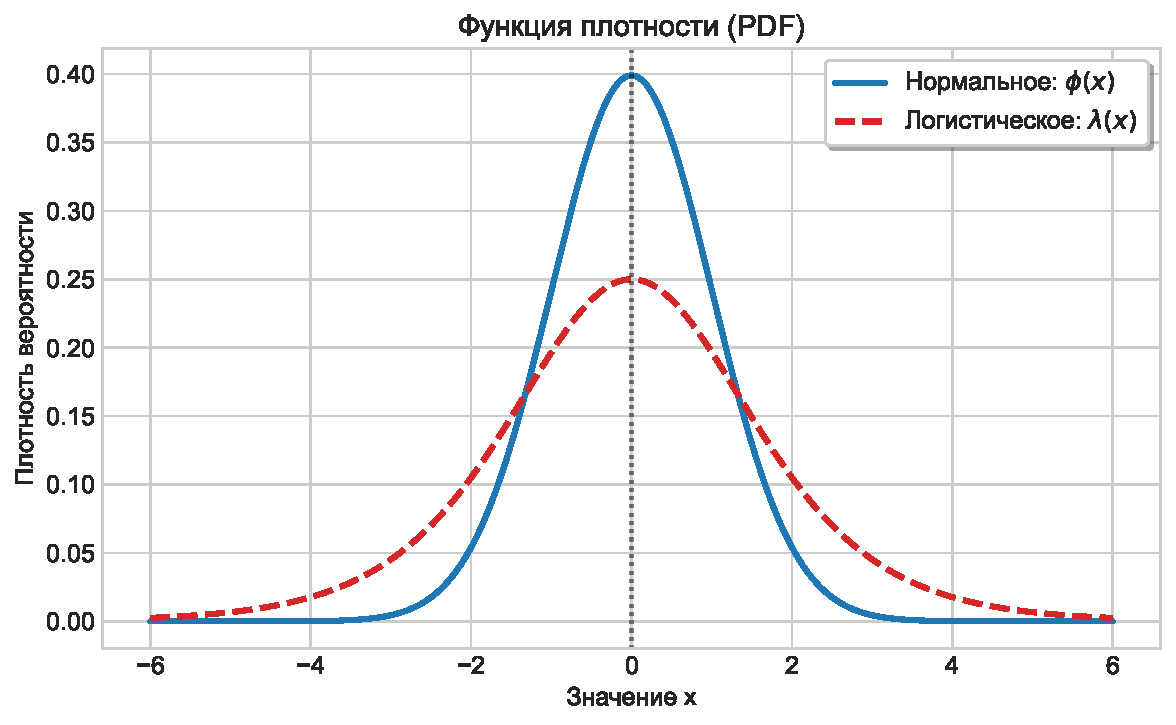
\includegraphics[keepaspectratio]{list22-logit_files/figure-pdf/cell-3-output-1.pdf}}

Функции распределения на одном графике

\pandocbounded{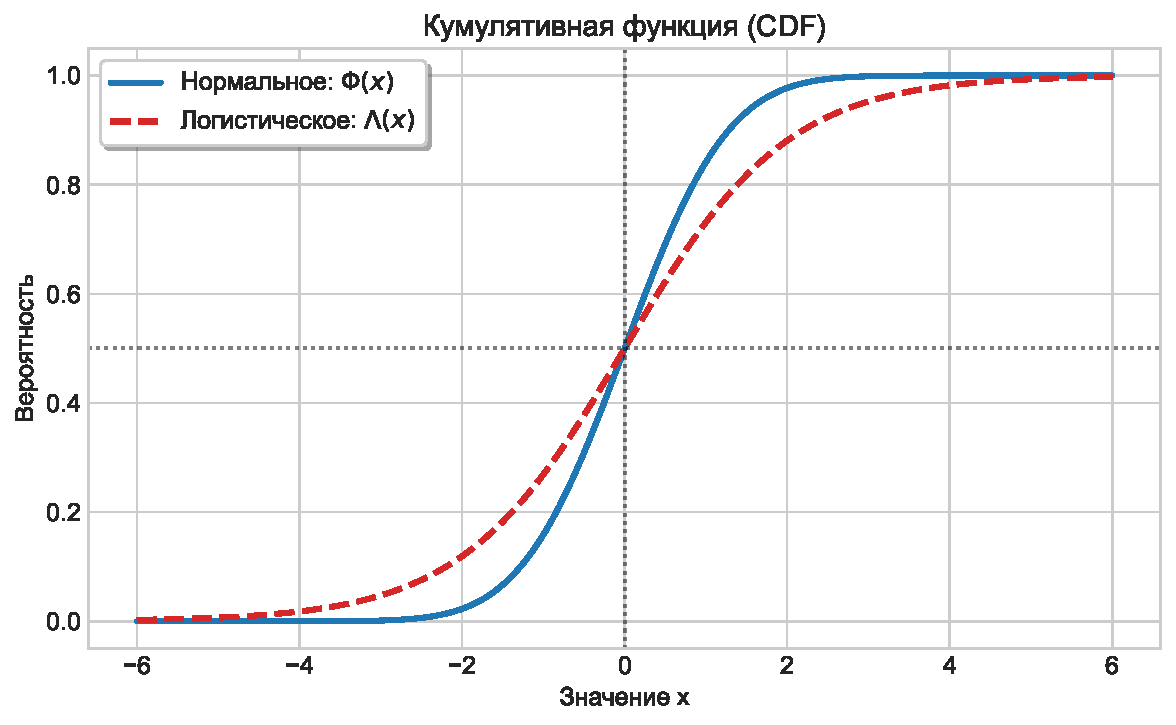
\includegraphics[keepaspectratio]{list22-logit_files/figure-pdf/cell-4-output-1.pdf}}

Обратные функции распределения

\[
logit(p)=\Lambda^{-1}(p)=\log\frac{p}{1-p} \quad \text{ и } \quad probit(p)=\Phi^{-1}(p), \quad 0<p<1
\]

Их графики

\pandocbounded{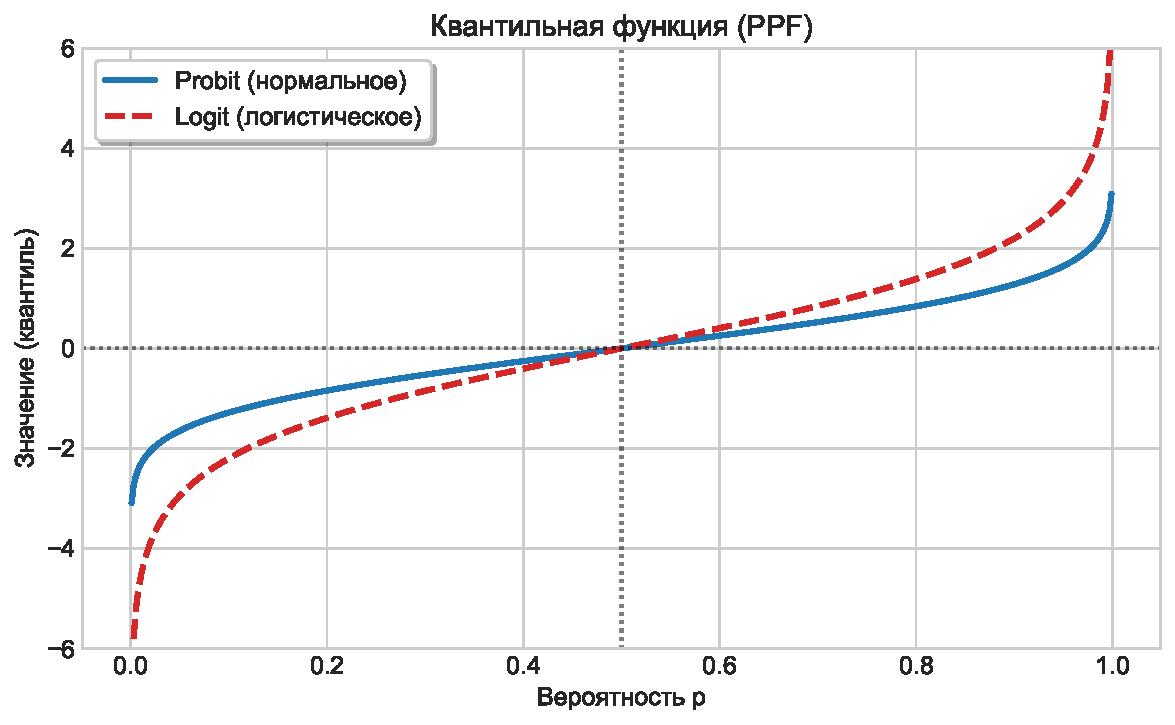
\includegraphics[keepaspectratio]{list22-logit_files/figure-pdf/cell-5-output-1.pdf}}

\section{Оценивание и интерпретация
коэффициентов}\label{ux43eux446ux435ux43dux438ux432ux430ux43dux438ux435-ux438-ux438ux43dux442ux435ux440ux43fux440ux435ux442ux430ux446ux438ux44f-ux43aux43eux44dux444ux444ux438ux446ux438ux435ux43dux442ux43eux432}

\subsection{approve equation \#1
(probit)}\label{approve-equation-1-probit}

Для датасета \texttt{loanapp} рассмотрим probit-регрессию
\textbf{approve на appinc, mortno, unem, dep, male, married, yjob, self}

Спецификация:

\[
P(approve=1)=\Phi(\beta_0+\beta_1appinc+\beta_2mortno+\beta_3unem+\beta_4dep+\beta_5male+\beta_6married+\beta_7yjob+\beta_8self)
\]

Альтернативная спецификация:

\[
probit(P(approve=1))=\beta_0+\beta_1appinc+\beta_2mortno+\beta_3unem+\beta_4dep+\beta_5male+\beta_6married+\beta_7yjob+\beta_8self
\]

Оцените модель на данных и укажите коэффициенты подогнанной модели.
\textbf{Ответ округлите до 3-х десятичных знаков.}

Ответ:

{\def\LTcaptype{none} % do not increment counter
\begin{longtable}[]{@{}lr@{}}
\toprule\noalign{}
Переменная & Оценка (MLE) \\
\midrule\noalign{}
\endhead
\bottomrule\noalign{}
\endlastfoot
Intercept & 1.142 \\
appinc & -0.001 \\
mortno & 0.407 \\
unem & -0.031 \\
dep & -0.083 \\
male & 0.02 \\
married & 0.221 \\
yjob & -0.001 \\
self & -0.158 \\
\end{longtable}
}

Дайте интерпретацию коэффициентам модели.

\subsection{approve equation \#2
(logit)}\label{approve-equation-2-logit}

Для датасета \texttt{loanapp} рассмотрим logit-регрессию \textbf{approve
на appinc, mortno, unem, dep, male, married, yjob, self}

Спецификация:

\[
P(approve=1)=\Lambda(\beta_0+\beta_1appinc+\beta_2mortno+\beta_3unem+\beta_4dep+\beta_5male+\beta_6married+\beta_7yjob+\beta_8self)
\]

Альтернативная спецификация:

\[
logit(P(approve=1))=\beta_0+\beta_1appinc+\beta_2mortno+\beta_3unem+\beta_4dep+\beta_5male+\beta_6married+\beta_7yjob+\beta_8self
\]

Здесь

\[
logit(P(approve=1)) = \log\frac{P(approve=1)}{1-P(approve=1)} = \log\frac{P(approve=1)}{P(approve=0)}
\]

Оцените модель на данных и укажите коэффициенты подогнанной модели.
\textbf{Ответ округлите до 3-х десятичных знаков.}

Ответ:

{\def\LTcaptype{none} % do not increment counter
\begin{longtable}[]{@{}lr@{}}
\toprule\noalign{}
Переменная & Оценка (MLE) \\
\midrule\noalign{}
\endhead
\bottomrule\noalign{}
\endlastfoot
Intercept & 1.931 \\
appinc & -0.001 \\
mortno & 0.787 \\
unem & -0.055 \\
dep & -0.161 \\
male & 0.03 \\
married & 0.425 \\
yjob & -0.006 \\
self & -0.28 \\
\end{longtable}
}

Дайте интерпретацию коэффициентам модели.

\subsection{labour force equation \#1
(probit)}\label{labour-force-equation-1-probit}

Для датасета \texttt{TableF5-1} рассмотрим probit-регрессию \textbf{LFP
на WA, I(WA ** 2), WE, KL6, K618, CIT, UN, np.log(FAMINC)}

Спецификация:

\[
P(LFP=1)=\Phi(\beta_0+\beta_1WA+\beta_2WA^2+\beta_3WE+\beta_4KL6+\beta_5K618+\beta_6CIT+\beta_7UN+\beta_8\log(FAMINC))
\]

Альтернативная спецификация:

\[
probit(P(LFP=1))=\beta_0+\beta_1WA+\beta_2WA^2+\beta_3WE+\beta_4KL6+\beta_5K618+\beta_6CIT+\beta_7UN+\beta_8\log(FAMINC)
\]

Оцените модель на данных и укажите коэффициенты подогнанной модели.
\textbf{Ответ округлите до 3-х десятичных знаков.}

Ответ:

{\def\LTcaptype{none} % do not increment counter
\begin{longtable}[]{@{}lr@{}}
\toprule\noalign{}
Переменная & Оценка (MLE) \\
\midrule\noalign{}
\endhead
\bottomrule\noalign{}
\endlastfoot
Intercept & -2.005 \\
WA & 0.008 \\
I(WA ** 2) & -0.001 \\
WE & 0.109 \\
KL6 & -0.851 \\
K618 & -0.063 \\
CIT & -0.128 \\
UN & -0.011 \\
np.log(FAMINC) & 0.2 \\
\end{longtable}
}

Дайте интерпретацию коэффициентам модели.

\subsection{labour force equation \#2
(logit)}\label{labour-force-equation-2-logit}

Для датасета \texttt{TableF5-1} рассмотрим logit-регрессию \textbf{LFP
на WA, I(WA ** 2), WE, KL6, K618, CIT, UN, np.log(FAMINC)}

Спецификация:

\[
P(LFP=1)=\Lambda(\beta_0+\beta_1WA+\beta_2WA^2+\beta_3WE+\beta_4KL6+\beta_5K618+\beta_6CIT+\beta_7UN+\beta_8\log(FAMINC))
\]

Альтернативная спецификация:

\[
logit(LFP)=\beta_0+\beta_1WA+\beta_2WA^2+\beta_3WE+\beta_4KL6+\beta_5K618+\beta_6CIT+\beta_7UN+\beta_8\log(FAMINC)
\]

Здесь

\[
logit(P(LFP=1)) = \log\frac{P(LFP=1)}{1-P(LFP=1)} = \log\frac{P(LFP=1)}{P(LFP=0)}
\]

Оцените модель на данных и укажите коэффициенты подогнанной модели.
\textbf{Ответ округлите до 3-х десятичных знаков.}

Ответ:

{\def\LTcaptype{none} % do not increment counter
\begin{longtable}[]{@{}lr@{}}
\toprule\noalign{}
Переменная & Оценка (MLE) \\
\midrule\noalign{}
\endhead
\bottomrule\noalign{}
\endlastfoot
Intercept & -3.241 \\
WA & 0.007 \\
I(WA ** 2) & -0.001 \\
WE & 0.18 \\
KL6 & -1.414 \\
K618 & -0.104 \\
CIT & -0.217 \\
UN & -0.018 \\
np.log(FAMINC) & 0.333 \\
\end{longtable}
}

Дайте интерпретацию коэффициентам модели.

\section{z-test}\label{z-test}

\subsection{approve equation \#1
(probit)}\label{approve-equation-1-probit-1}

Для датасета \texttt{loanapp} рассмотрим probit-регрессию
\textbf{approve на appinc, mortno, unem, dep, male, married, yjob, self}

Подгоните модель на данных и приведите результаты \(z\)-теста

Ответ:

{\def\LTcaptype{none} % do not increment counter
\begin{longtable}[]{@{}lrrrrl@{}}
\toprule\noalign{}
& Coef. & Std.Err. & z-value & p-value & Signif. \\
\midrule\noalign{}
\endhead
\bottomrule\noalign{}
\endlastfoot
Intercept & 1.1418 & 0.1086 & 10.5122 & 0 & \\
appinc & -0.0005 & 0.0004 & -1.3752 & 0.1691 & \\
mortno & 0.4071 & 0.0866 & 4.7026 & 0 & *** \\
unem & -0.0308 & 0.0161 & -1.9086 & 0.0563 & * \\
dep & -0.0828 & 0.0352 & -2.3546 & 0.0185 & ** \\
male & 0.02 & 0.0995 & 0.2009 & 0.8408 & \\
married & 0.2208 & 0.0865 & 2.5522 & 0.0107 & ** \\
yjob & -0.0007 & 0.0349 & -0.02 & 0.984 & \\
self & -0.1583 & 0.1067 & -1.4826 & 0.1382 & \\
\end{longtable}
}

\emph{Signif. codes:} \texttt{***} \(p<0.01\), \texttt{**} \(p<0.05\),
\texttt{*} \(p<0.1\)

Модель была подогнана по 1971 наблюдениям. {Уровень значимости 10\%}

Вычислите необходимое критическое значение \(z\)-теста. \textbf{Ответ
округлите до 3-х десятичных знаков.}

\begin{tcolorbox}[enhanced jigsaw, arc=.35mm, bottomrule=.15mm, bottomtitle=1mm, breakable, colback=white, colbacktitle=quarto-callout-note-color!10!white, colframe=quarto-callout-note-color-frame, coltitle=black, left=2mm, leftrule=.75mm, opacityback=0, opacitybacktitle=0.6, rightrule=.15mm, title=\textcolor{quarto-callout-note-color}{\faInfo}\hspace{0.5em}{Критическое значение z-теста}, titlerule=0mm, toprule=.15mm, toptitle=1mm]

\(z_{crit} = 1.645\)

\end{tcolorbox}

Какие коэффициенты значимы?

\begin{tcolorbox}[enhanced jigsaw, arc=.35mm, bottomrule=.15mm, bottomtitle=1mm, breakable, colback=white, colbacktitle=quarto-callout-note-color!10!white, colframe=quarto-callout-note-color-frame, coltitle=black, left=2mm, leftrule=.75mm, opacityback=0, opacitybacktitle=0.6, rightrule=.15mm, title=\textcolor{quarto-callout-note-color}{\faInfo}\hspace{0.5em}{Коэффициенты, значимые на уровне 10\% (по классическим стандартным
ошибкам)}, titlerule=0mm, toprule=.15mm, toptitle=1mm]

\texttt{mortno}, \texttt{unem}, \texttt{dep}, \texttt{married}

\end{tcolorbox}

\subsection{approve equation \#2
(logit)}\label{approve-equation-2-logit-1}

Для датасета \texttt{loanapp} рассмотрим logit-регрессию \textbf{approve
на appinc, mortno, unem, dep, male, married, yjob, self}

Подгоните модель на данных и приведите результаты \(z\)-теста

Ответ:

{\def\LTcaptype{none} % do not increment counter
\begin{longtable}[]{@{}lrrrrl@{}}
\toprule\noalign{}
& Coef. & Std.Err. & z-value & p-value & Signif. \\
\midrule\noalign{}
\endhead
\bottomrule\noalign{}
\endlastfoot
Intercept & 1.9315 & 0.1993 & 9.6891 & 0 & \\
appinc & -0.001 & 0.0007 & -1.4717 & 0.1411 & \\
mortno & 0.7868 & 0.1721 & 4.5714 & 0 & *** \\
unem & -0.0549 & 0.0294 & -1.8661 & 0.062 & * \\
dep & -0.1608 & 0.0647 & -2.4861 & 0.0129 & ** \\
male & 0.03 & 0.1859 & 0.1612 & 0.8719 & \\
married & 0.4246 & 0.1624 & 2.6145 & 0.0089 & *** \\
yjob & -0.0065 & 0.0651 & -0.0993 & 0.9209 & \\
self & -0.2804 & 0.1967 & -1.4257 & 0.1539 & \\
\end{longtable}
}

\emph{Signif. codes:} \texttt{***} \(p<0.01\), \texttt{**} \(p<0.05\),
\texttt{*} \(p<0.1\)

Модель была подогнана по 1971 наблюдениям. {Уровень значимости 5\%}

Вычислите необходимое критическое значение \(z\)-теста. \textbf{Ответ
округлите до 3-х десятичных знаков.}

\begin{tcolorbox}[enhanced jigsaw, arc=.35mm, bottomrule=.15mm, bottomtitle=1mm, breakable, colback=white, colbacktitle=quarto-callout-note-color!10!white, colframe=quarto-callout-note-color-frame, coltitle=black, left=2mm, leftrule=.75mm, opacityback=0, opacitybacktitle=0.6, rightrule=.15mm, title=\textcolor{quarto-callout-note-color}{\faInfo}\hspace{0.5em}{Критическое значение z-теста}, titlerule=0mm, toprule=.15mm, toptitle=1mm]

\(z_{crit} = 1.960\)

\end{tcolorbox}

Какие коэффициенты значимы?

\begin{tcolorbox}[enhanced jigsaw, arc=.35mm, bottomrule=.15mm, bottomtitle=1mm, breakable, colback=white, colbacktitle=quarto-callout-note-color!10!white, colframe=quarto-callout-note-color-frame, coltitle=black, left=2mm, leftrule=.75mm, opacityback=0, opacitybacktitle=0.6, rightrule=.15mm, title=\textcolor{quarto-callout-note-color}{\faInfo}\hspace{0.5em}{Коэффициенты, значимые на уровне 5\% (по классическим стандартным
ошибкам)}, titlerule=0mm, toprule=.15mm, toptitle=1mm]

\texttt{mortno}, \texttt{dep}, \texttt{married}

\end{tcolorbox}

\subsection{labour force equation \#1
(probit)}\label{labour-force-equation-1-probit-1}

Для датасета \texttt{TableF5-1} рассмотрим probit-регрессию \textbf{LFP
на WA, I(WA ** 2), WE, KL6, K618, CIT, UN, np.log(FAMINC)}

Подгоните модель на данных и приведите результаты z-теста

Ответ:

{\def\LTcaptype{none} % do not increment counter
\begin{longtable}[]{@{}
  >{\raggedright\arraybackslash}p{(\linewidth - 10\tabcolsep) * \real{0.2286}}
  >{\raggedleft\arraybackslash}p{(\linewidth - 10\tabcolsep) * \real{0.1286}}
  >{\raggedleft\arraybackslash}p{(\linewidth - 10\tabcolsep) * \real{0.1714}}
  >{\raggedleft\arraybackslash}p{(\linewidth - 10\tabcolsep) * \real{0.1571}}
  >{\raggedleft\arraybackslash}p{(\linewidth - 10\tabcolsep) * \real{0.1571}}
  >{\raggedright\arraybackslash}p{(\linewidth - 10\tabcolsep) * \real{0.1571}}@{}}
\toprule\noalign{}
\begin{minipage}[b]{\linewidth}\raggedright
\end{minipage} & \begin{minipage}[b]{\linewidth}\raggedleft
Coef.
\end{minipage} & \begin{minipage}[b]{\linewidth}\raggedleft
Std.Err.
\end{minipage} & \begin{minipage}[b]{\linewidth}\raggedleft
z-value
\end{minipage} & \begin{minipage}[b]{\linewidth}\raggedleft
p-value
\end{minipage} & \begin{minipage}[b]{\linewidth}\raggedright
Signif.
\end{minipage} \\
\midrule\noalign{}
\endhead
\bottomrule\noalign{}
\endlastfoot
Intercept & -2.0046 & 1.7055 & -1.1754 & 0.2398 & \\
WA & 0.0076 & 0.0703 & 0.1084 & 0.9137 & \\
I(WA ** 2) & -0.0005 & 0.0008 & -0.6538 & 0.5132 & \\
WE & 0.1088 & 0.0241 & 4.514 & 0 & *** \\
KL6 & -0.8513 & 0.1146 & -7.4277 & 0 & *** \\
K618 & -0.0632 & 0.0415 & -1.5206 & 0.1284 & \\
CIT & -0.1277 & 0.1074 & -1.1891 & 0.2344 & \\
UN & -0.0106 & 0.0157 & -0.6785 & 0.4975 & \\
np.log(FAMINC) & 0.1996 & 0.1046 & 1.9081 & 0.0564 & * \\
\end{longtable}
}

\emph{Signif. codes:} \texttt{***} \(p<0.01\), \texttt{**} \(p<0.05\),
\texttt{*} \(p<0.1\)

Модель была подогнана по 753 наблюдениям. {Уровень значимости 10\%}

Вычислите необходимое критическое значение \(z\)-теста. \textbf{Ответ
округлите до 3-х десятичных знаков.}

\begin{tcolorbox}[enhanced jigsaw, arc=.35mm, bottomrule=.15mm, bottomtitle=1mm, breakable, colback=white, colbacktitle=quarto-callout-note-color!10!white, colframe=quarto-callout-note-color-frame, coltitle=black, left=2mm, leftrule=.75mm, opacityback=0, opacitybacktitle=0.6, rightrule=.15mm, title=\textcolor{quarto-callout-note-color}{\faInfo}\hspace{0.5em}{Критическое значение z-теста}, titlerule=0mm, toprule=.15mm, toptitle=1mm]

\(z_{crit} = 1.645\)

\end{tcolorbox}

Какие коэффициенты значимы?

\begin{tcolorbox}[enhanced jigsaw, arc=.35mm, bottomrule=.15mm, bottomtitle=1mm, breakable, colback=white, colbacktitle=quarto-callout-note-color!10!white, colframe=quarto-callout-note-color-frame, coltitle=black, left=2mm, leftrule=.75mm, opacityback=0, opacitybacktitle=0.6, rightrule=.15mm, title=\textcolor{quarto-callout-note-color}{\faInfo}\hspace{0.5em}{Коэффициенты, значимые на уровне 10\% (по классическим стандартным
ошибкам)}, titlerule=0mm, toprule=.15mm, toptitle=1mm]

\texttt{WE}, \texttt{KL6}, \texttt{np.log(FAMINC)}

\end{tcolorbox}

\subsection{labour force equation \#2
(logit)}\label{labour-force-equation-2-logit-1}

Для датасета \texttt{TableF5-1} рассмотрим logit-регрессию \textbf{LFP
на WA, I(WA ** 2), WE, KL6, K618, CIT, UN, np.log(FAMINC)}

Подгоните модель на данных и приведите результаты \(z\)-теста

Ответ:

{\def\LTcaptype{none} % do not increment counter
\begin{longtable}[]{@{}
  >{\raggedright\arraybackslash}p{(\linewidth - 10\tabcolsep) * \real{0.2286}}
  >{\raggedleft\arraybackslash}p{(\linewidth - 10\tabcolsep) * \real{0.1286}}
  >{\raggedleft\arraybackslash}p{(\linewidth - 10\tabcolsep) * \real{0.1714}}
  >{\raggedleft\arraybackslash}p{(\linewidth - 10\tabcolsep) * \real{0.1571}}
  >{\raggedleft\arraybackslash}p{(\linewidth - 10\tabcolsep) * \real{0.1571}}
  >{\raggedright\arraybackslash}p{(\linewidth - 10\tabcolsep) * \real{0.1571}}@{}}
\toprule\noalign{}
\begin{minipage}[b]{\linewidth}\raggedright
\end{minipage} & \begin{minipage}[b]{\linewidth}\raggedleft
Coef.
\end{minipage} & \begin{minipage}[b]{\linewidth}\raggedleft
Std.Err.
\end{minipage} & \begin{minipage}[b]{\linewidth}\raggedleft
z-value
\end{minipage} & \begin{minipage}[b]{\linewidth}\raggedleft
p-value
\end{minipage} & \begin{minipage}[b]{\linewidth}\raggedright
Signif.
\end{minipage} \\
\midrule\noalign{}
\endhead
\bottomrule\noalign{}
\endlastfoot
Intercept & -3.2407 & 2.8337 & -1.1436 & 0.2528 & \\
WA & 0.007 & 0.1159 & 0.0602 & 0.952 & \\
I(WA ** 2) & -0.0008 & 0.0013 & -0.6061 & 0.5444 & \\
WE & 0.18 & 0.0404 & 4.4535 & 0 & *** \\
KL6 & -1.4138 & 0.1987 & -7.1152 & 0 & *** \\
K618 & -0.1042 & 0.0687 & -1.5166 & 0.1294 & \\
CIT & -0.2165 & 0.1765 & -1.2267 & 0.2199 & \\
UN & -0.0176 & 0.0258 & -0.6812 & 0.4957 & \\
np.log(FAMINC) & 0.3331 & 0.1729 & 1.9272 & 0.054 & * \\
\end{longtable}
}

\emph{Signif. codes:} \texttt{***} \(p<0.01\), \texttt{**} \(p<0.05\),
\texttt{*} \(p<0.1\)

Модель была подогнана по 753 наблюдениям. {Уровень значимости 5\%}

Вычислите необходимое критическое значение \(z\)-теста. \textbf{Ответ
округлите до 3-х десятичных знаков.}

\begin{tcolorbox}[enhanced jigsaw, arc=.35mm, bottomrule=.15mm, bottomtitle=1mm, breakable, colback=white, colbacktitle=quarto-callout-note-color!10!white, colframe=quarto-callout-note-color-frame, coltitle=black, left=2mm, leftrule=.75mm, opacityback=0, opacitybacktitle=0.6, rightrule=.15mm, title=\textcolor{quarto-callout-note-color}{\faInfo}\hspace{0.5em}{Критическое значение z-теста}, titlerule=0mm, toprule=.15mm, toptitle=1mm]

\(z_{crit} = 1.960\)

\end{tcolorbox}

Какие коэффициенты значимы?

\begin{tcolorbox}[enhanced jigsaw, arc=.35mm, bottomrule=.15mm, bottomtitle=1mm, breakable, colback=white, colbacktitle=quarto-callout-note-color!10!white, colframe=quarto-callout-note-color-frame, coltitle=black, left=2mm, leftrule=.75mm, opacityback=0, opacitybacktitle=0.6, rightrule=.15mm, title=\textcolor{quarto-callout-note-color}{\faInfo}\hspace{0.5em}{Коэффициенты, значимые на уровне 5\% (по классическим стандартным
ошибкам)}, titlerule=0mm, toprule=.15mm, toptitle=1mm]

\texttt{WE}, \texttt{KL6}

\end{tcolorbox}

\section{LR-тест: значимость
регрессии}\label{lr-ux442ux435ux441ux442-ux437ux43dux430ux447ux438ux43cux43eux441ux442ux44c-ux440ux435ux433ux440ux435ux441ux441ux438ux438}

\subsection{approve equation \#1
(probit)}\label{approve-equation-1-probit-2}

Для датасета \texttt{loanapp} рассмотрим probit-регрессию
\textbf{approve на appinc, unem, male, yjob, self}

Подгоните модель на данных и укажите:

\begin{itemize}
\tightlist
\item
  число наблюдений, на которых была подогнана модель
\item
  логарифм функции правдоподобия для модели \(\log L\)
\item
  логарифм функции правдоподобия для регрессии без объясняющих
  переменных (только на константу)
\end{itemize}

\textbf{Ответ округлите до 4-х десятичных знаков}.

\textbf{Ответ:}

\begin{itemize}
\tightlist
\item
  число наблюдений: 1971
\item
  логарифм функции правдоподобия: \(\log L = -733.7270\)
\item
  логарифм функции правдоподобия для регрессии на константу:
  \(\log L_{null} = -737.9793\)
\end{itemize}

Тестируется значимость регрессии, т.е. гипотеза
\(H_0:\beta_{appinc}=\beta_{unem}=\beta_{male}=\beta_{yjob}=\beta_{self}=0\).
{Уровень значимости 10\%.}

Вычислите тестовую статистику. \textbf{Ответ округлите до 3-х десятичных
знаков.}

\begin{tcolorbox}[enhanced jigsaw, arc=.35mm, bottomrule=.15mm, bottomtitle=1mm, breakable, colback=white, colbacktitle=quarto-callout-note-color!10!white, colframe=quarto-callout-note-color-frame, coltitle=black, left=2mm, leftrule=.75mm, opacityback=0, opacitybacktitle=0.6, rightrule=.15mm, title=\textcolor{quarto-callout-note-color}{\faInfo}\hspace{0.5em}{LR Статистика}, titlerule=0mm, toprule=.15mm, toptitle=1mm]

\(LR = 8.505\)

\end{tcolorbox}

Вычислите критическое значение. \textbf{Ответ округлите до 3-х
десятичных знаков.}

\begin{tcolorbox}[enhanced jigsaw, arc=.35mm, bottomrule=.15mm, bottomtitle=1mm, breakable, colback=white, colbacktitle=quarto-callout-note-color!10!white, colframe=quarto-callout-note-color-frame, coltitle=black, left=2mm, leftrule=.75mm, opacityback=0, opacitybacktitle=0.6, rightrule=.15mm, title=\textcolor{quarto-callout-note-color}{\faInfo}\hspace{0.5em}{Критическое значение}, titlerule=0mm, toprule=.15mm, toptitle=1mm]

\(\chi^2_{crit} = 9.236\)

\end{tcolorbox}

Значима ли регрессия?

\begin{tcolorbox}[enhanced jigsaw, arc=.35mm, bottomrule=.15mm, bottomtitle=1mm, breakable, colback=white, colbacktitle=quarto-callout-important-color!10!white, colframe=quarto-callout-important-color-frame, coltitle=black, left=2mm, leftrule=.75mm, opacityback=0, opacitybacktitle=0.6, rightrule=.15mm, title=\textcolor{quarto-callout-important-color}{\faExclamation}\hspace{0.5em}{Вывод}, titlerule=0mm, toprule=.15mm, toptitle=1mm]

Регрессия \textbf{незначима}.

\end{tcolorbox}

Какие коэффициенты значимы?

\begin{tcolorbox}[enhanced jigsaw, arc=.35mm, bottomrule=.15mm, bottomtitle=1mm, breakable, colback=white, colbacktitle=quarto-callout-note-color!10!white, colframe=quarto-callout-note-color-frame, coltitle=black, left=2mm, leftrule=.75mm, opacityback=0, opacitybacktitle=0.6, rightrule=.15mm, title=\textcolor{quarto-callout-note-color}{\faInfo}\hspace{0.5em}{Коэффициенты, значимые на уровне 10\% (по классическим стандартным
ошибкам)}, titlerule=0mm, toprule=.15mm, toptitle=1mm]

\texttt{unem}

\end{tcolorbox}

\subsection{approve equation \#2
(logit)}\label{approve-equation-2-logit-2}

Для датасета \texttt{loanapp} рассмотрим logit-регрессию \textbf{approve
на appinc, appinc ** 2, mortno, unem, dep, male, married, yjob, self}

Подгоните модель на данных и укажите:

\begin{itemize}
\tightlist
\item
  число наблюдений, на которых была подогнана модель
\item
  логарифм функции правдоподобия для модели \(\log L\)
\item
  логарифм функции правдоподобия для регрессии без объясняющих
  переменных (только на константу)
\end{itemize}

\textbf{Ответ округлите до 4-х десятичных знаков.}

\textbf{Ответ:}

\begin{itemize}
\tightlist
\item
  число наблюдений: 1971
\item
  логарифм функции правдоподобия: \(\log L = -713.7313\)
\item
  логарифм функции правдоподобия для регрессии на константу:
  \(\log L_{null} = -737.9793\)
\end{itemize}

Тестируется значимость регрессии, т.е. гипотеза
\(H_0:\beta_{appinc}=\beta_{unem}=\beta_{male}=\beta_{yjob}=\beta_{self}=0\).
{Уровень значимости 5\%}.

Вычислите тестовую статистику. \textbf{Ответ округлите до 3-х десятичных
знаков.}

\begin{tcolorbox}[enhanced jigsaw, arc=.35mm, bottomrule=.15mm, bottomtitle=1mm, breakable, colback=white, colbacktitle=quarto-callout-note-color!10!white, colframe=quarto-callout-note-color-frame, coltitle=black, left=2mm, leftrule=.75mm, opacityback=0, opacitybacktitle=0.6, rightrule=.15mm, title=\textcolor{quarto-callout-note-color}{\faInfo}\hspace{0.5em}{LR-статистика}, titlerule=0mm, toprule=.15mm, toptitle=1mm]

\(LR = 48.496\)

\end{tcolorbox}

Вычислите критическое значение. \textbf{Ответ округлите до 3-х
десятичных знаков.}

\begin{tcolorbox}[enhanced jigsaw, arc=.35mm, bottomrule=.15mm, bottomtitle=1mm, breakable, colback=white, colbacktitle=quarto-callout-note-color!10!white, colframe=quarto-callout-note-color-frame, coltitle=black, left=2mm, leftrule=.75mm, opacityback=0, opacitybacktitle=0.6, rightrule=.15mm, title=\textcolor{quarto-callout-note-color}{\faInfo}\hspace{0.5em}{Критическое значение}, titlerule=0mm, toprule=.15mm, toptitle=1mm]

\(\chi^2_{crit} = 16.919\)

\end{tcolorbox}

Значима ли регрессия?

\begin{tcolorbox}[enhanced jigsaw, arc=.35mm, bottomrule=.15mm, bottomtitle=1mm, breakable, colback=white, colbacktitle=quarto-callout-tip-color!10!white, colframe=quarto-callout-tip-color-frame, coltitle=black, left=2mm, leftrule=.75mm, opacityback=0, opacitybacktitle=0.6, rightrule=.15mm, title=\textcolor{quarto-callout-tip-color}{\faLightbulb}\hspace{0.5em}{Вывод}, titlerule=0mm, toprule=.15mm, toptitle=1mm]

Регрессия \textbf{значима}.

\end{tcolorbox}

Какие коэффициенты значимы?

\begin{tcolorbox}[enhanced jigsaw, arc=.35mm, bottomrule=.15mm, bottomtitle=1mm, breakable, colback=white, colbacktitle=quarto-callout-note-color!10!white, colframe=quarto-callout-note-color-frame, coltitle=black, left=2mm, leftrule=.75mm, opacityback=0, opacitybacktitle=0.6, rightrule=.15mm, title=\textcolor{quarto-callout-note-color}{\faInfo}\hspace{0.5em}{Коэффициенты, значимые на уровне 5\% (по классическим стандартным
ошибкам)}, titlerule=0mm, toprule=.15mm, toptitle=1mm]

\texttt{I(appinc\ **\ 2)}, \texttt{mortno}, \texttt{dep},
\texttt{married}

\end{tcolorbox}

\subsection{labour force equation \#1
(probit)}\label{labour-force-equation-1-probit-2}

Для датасета \texttt{TableF5-1} рассмотрим несколько probit-регрессий:

\begin{itemize}
\tightlist
\item
  Модель 1: \textbf{LFP на WA, I(WA ** 2), WE, KL6, K618, CIT, UN,
  np.log(FAMINC)}
\item
  Модель 2: \textbf{LFP на WA, I(WA ** 2), CIT, UN, np.log(FAMINC)}
\item
  Модель 3: \textbf{LFP на WA, I(WA ** 2), CIT, UN}
\item
  Модель 4: \textbf{LFP на CIT, UN}
\end{itemize}

Результаты оценивания:

{\def\LTcaptype{none} % do not increment counter
\begin{longtable}[]{@{}lllll@{}}
\toprule\noalign{}
& Model 1 & Model 2 & Model 3 & Model 4 \\
\midrule\noalign{}
\endhead
\bottomrule\noalign{}
\endlastfoot
Dep. Variable & LFP & LFP & LFP & LFP \\
WA & 0.0076 & 0.1084* & 0.1297** & \\
& (0.0703) & (0.0632) & (0.0629) & \\
I(WA ** 2) & -0.0005 & -0.0014* & -0.0016** & \\
& (0.0008) & (0.0007) & (0.0007) & \\
WE & 0.1088*** & & & \\
& (0.0241) & & & \\
KL6 & -0.8513*** & & & \\
& (0.1146) & & & \\
K618 & -0.0632 & & & \\
& (0.0415) & & & \\
CIT & -0.1277 & -0.1026 & 0.0053 & -0.0024 \\
& (0.1074) & (0.1030) & (0.0984) & (0.0975) \\
UN & -0.0106 & -0.0101 & -0.0102 & -0.0115 \\
& (0.0157) & (0.0151) & (0.0151) & (0.0150) \\
np.log(FAMINC) & 0.1996* & 0.3621*** & & \\
& (0.1046) & (0.0946) & & \\
Intercept & -2.0046 & -5.2366*** & -2.1745 & 0.2733* \\
& (1.7055) & (1.5554) & (1.3261) & (0.1407) \\
Log-Likelihood & -462.340 & -502.224 & -509.653 & -514.563 \\
Nobs & 753 & 753 & 753 & 753 \\
\end{longtable}
}

\emph{Signif. codes:} *** \(p<0.01\), ** \(p<0.05\), * \(p<0.1\)

Для каждой регрессии вычислите LR-статистику для тестирования её
значимости. \textbf{Ответ округлите до 3-х десятичных знаков.}

{\def\LTcaptype{none} % do not increment counter
\begin{longtable}[]{@{}rr@{}}
\toprule\noalign{}
Регрессия & LR-статистика \\
\midrule\noalign{}
\endhead
\bottomrule\noalign{}
\endlastfoot
1 & 105.066 \\
2 & 25.299 \\
3 & 10.44 \\
4 & 0.62 \\
\end{longtable}
}

Для каждой регрессии вычислите необходимое критическое значение.
{Уровень значимости 10\%}. \textbf{Ответ округлите до 3-х десятичных
знаков.}

{\def\LTcaptype{none} % do not increment counter
\begin{longtable}[]{@{}rr@{}}
\toprule\noalign{}
Регрессия & Критическое значение \\
\midrule\noalign{}
\endhead
\bottomrule\noalign{}
\endlastfoot
1 & 13.362 \\
2 & 9.236 \\
3 & 7.779 \\
4 & 4.605 \\
\end{longtable}
}

Какая из регрессий значима?

{\def\LTcaptype{none} % do not increment counter
\begin{longtable}[]{@{}rl@{}}
\toprule\noalign{}
Регрессия & Значимость \\
\midrule\noalign{}
\endhead
\bottomrule\noalign{}
\endlastfoot
1 & Значима \\
2 & Значима \\
3 & Значима \\
4 & Незначима \\
\end{longtable}
}

\subsection{labour force equation \#2
(logit)}\label{labour-force-equation-2-logit-2}

Для датасета \texttt{TableF5-1} рассмотрим несколько logit-регрессий:

\begin{itemize}
\tightlist
\item
  Модель 1: \textbf{LFP на WA, I(WA ** 2), WE, KL6, K618, CIT, UN,
  np.log(FAMINC)}
\item
  Модель 2: \textbf{LFP на WE, KL6, K618, CIT, UN, np.log(FAMINC)}
\item
  Модель 3: \textbf{LFP на KL6, K618, CIT, UN, np.log(FAMINC)}
\item
  Модель 4: \textbf{LFP на K618, CIT, UN}
\end{itemize}

Результаты оценивания:

{\def\LTcaptype{none} % do not increment counter
\begin{longtable}[]{@{}lllll@{}}
\toprule\noalign{}
& Model 1 & Model 2 & Model 3 & Model 4 \\
\midrule\noalign{}
\endhead
\bottomrule\noalign{}
\endlastfoot
Dep. Variable & LFP & LFP & LFP & LFP \\
WA & 0.0070 & & & \\
& (0.1159) & & & \\
I(WA ** 2) & -0.0008 & & & \\
& (0.0013) & & & \\
WE & 0.1800*** & 0.2028*** & & \\
& (0.0404) & (0.0396) & & \\
KL6 & -1.4138*** & -1.0154*** & -0.8645*** & \\
& (0.1987) & (0.1646) & (0.1585) & \\
K618 & -0.1042 & 0.0509 & 0.0288 & -0.0031 \\
& (0.0687) & (0.0594) & (0.0581) & (0.0558) \\
CIT & -0.2165 & -0.2753 & -0.2200 & -0.0043 \\
& (0.1765) & (0.1726) & (0.1691) & (0.1564) \\
UN & -0.0176 & -0.0287 & -0.0196 & -0.0185 \\
& (0.0258) & (0.0254) & (0.0248) & (0.0240) \\
np.log(FAMINC) & 0.3331* & 0.2808* & 0.5829*** & \\
& (0.1729) & (0.1683) & (0.1580) & \\
Intercept & -3.2407 & -4.3882*** & -5.0277*** & 0.4420* \\
& (2.8337) & (1.5718) & (1.5542) & (0.2383) \\
Log-Likelihood & -462.236 & -475.674 & -489.791 & -514.560 \\
Nobs & 753 & 753 & 753 & 753 \\
\end{longtable}
}

\emph{Signif. codes:} *** \(p<0.01\), ** \(p<0.05\), * \(p<0.1\)

Для каждой регрессии вычислите LR-статистику для тестирования её
значимости. \textbf{Ответ округлите до 3-х десятичных знаков.}

{\def\LTcaptype{none} % do not increment counter
\begin{longtable}[]{@{}rr@{}}
\toprule\noalign{}
Регрессия & LR stat \\
\midrule\noalign{}
\endhead
\bottomrule\noalign{}
\endlastfoot
1 & 105.274 \\
2 & 78.399 \\
3 & 50.165 \\
4 & 0.625 \\
\end{longtable}
}

Для каждой регрессии вычислите необходимое критическое значение {Уровень
значимости 5\%}. \textbf{Ответ округлите до 3-х десятичных знаков.}

{\def\LTcaptype{none} % do not increment counter
\begin{longtable}[]{@{}rr@{}}
\toprule\noalign{}
Регрессия & Критическое \\
\midrule\noalign{}
\endhead
\bottomrule\noalign{}
\endlastfoot
1 & 15.507 \\
2 & 12.592 \\
3 & 11.07 \\
4 & 7.815 \\
\end{longtable}
}

Какая из регрессий значима?

{\def\LTcaptype{none} % do not increment counter
\begin{longtable}[]{@{}rl@{}}
\toprule\noalign{}
Регрессия & Значимость \\
\midrule\noalign{}
\endhead
\bottomrule\noalign{}
\endlastfoot
1 & Значима \\
2 & Значима \\
3 & Значима \\
4 & Незначима \\
\end{longtable}
}

\section{LR-тест: совместная
значимость}\label{lr-ux442ux435ux441ux442-ux441ux43eux432ux43cux435ux441ux442ux43dux430ux44f-ux437ux43dux430ux447ux438ux43cux43eux441ux442ux44c}

\subsection{labour force equation \#1
(probit)}\label{labour-force-equation-1-probit-3}

Для датасета \texttt{TableF5-1} рассмотрим probit-регрессию \textbf{LFP
на WA, WA ** 2, WE, KL6, K618, CIT, UN, np.log(FAMINC)}

Оцените регрессию на данных и тестируйте следующие гипотезы, используя
LR-статистику. {Уровень значимости 10\%}.

\subsubsection{Гипотеза
1}\label{ux433ux438ux43fux43eux442ux435ux437ux430-1}

Тестируется значимость влияния возраста, т.е. гипотеза
\(H_0:\beta_{WA}=\beta_{WA^2}=0\) по LR-тесту.

Вычислите соответствующую тестовую статистику. \textbf{Ответ округлите
до 3-х десятичных знаков.}

\begin{tcolorbox}[enhanced jigsaw, arc=.35mm, bottomrule=.15mm, bottomtitle=1mm, breakable, colback=white, colbacktitle=quarto-callout-note-color!10!white, colframe=quarto-callout-note-color-frame, coltitle=black, left=2mm, leftrule=.75mm, opacityback=0, opacitybacktitle=0.6, rightrule=.15mm, title=\textcolor{quarto-callout-note-color}{\faInfo}\hspace{0.5em}{LR-статистика}, titlerule=0mm, toprule=.15mm, toptitle=1mm]

\(LR = 26.718\)

\end{tcolorbox}

Вычислите необходимое критическое значение. \textbf{Ответ округлите до
3-х десятичных знаков.}

\begin{tcolorbox}[enhanced jigsaw, arc=.35mm, bottomrule=.15mm, bottomtitle=1mm, breakable, colback=white, colbacktitle=quarto-callout-note-color!10!white, colframe=quarto-callout-note-color-frame, coltitle=black, left=2mm, leftrule=.75mm, opacityback=0, opacitybacktitle=0.6, rightrule=.15mm, title=\textcolor{quarto-callout-note-color}{\faInfo}\hspace{0.5em}{Критическое значение}, titlerule=0mm, toprule=.15mm, toptitle=1mm]

\(\chi^2_{crit} = 4.605\)

\end{tcolorbox}

Значимо ли влияние возраста?

\begin{tcolorbox}[enhanced jigsaw, arc=.35mm, bottomrule=.15mm, bottomtitle=1mm, breakable, colback=white, colbacktitle=quarto-callout-tip-color!10!white, colframe=quarto-callout-tip-color-frame, coltitle=black, left=2mm, leftrule=.75mm, opacityback=0, opacitybacktitle=0.6, rightrule=.15mm, title=\textcolor{quarto-callout-tip-color}{\faLightbulb}\hspace{0.5em}{Вывод}, titlerule=0mm, toprule=.15mm, toptitle=1mm]

Влияние возраста \textbf{значимо}.

\end{tcolorbox}

\subsubsection{Гипотеза
2}\label{ux433ux438ux43fux43eux442ux435ux437ux430-2}

Тестируется совместная значимость влияния \textbf{K618, CIT, UN}, т.е.
гипотеза \(H_0:\beta_{K618}=\beta_{CIT}=\beta_{UN}=0\) по LR-тесту.

Вычислите соотвествующую тестовую статистику. \textbf{Ответ округлите до
3-х десятичных знаков.}

\begin{tcolorbox}[enhanced jigsaw, arc=.35mm, bottomrule=.15mm, bottomtitle=1mm, breakable, colback=white, colbacktitle=quarto-callout-note-color!10!white, colframe=quarto-callout-note-color-frame, coltitle=black, left=2mm, leftrule=.75mm, opacityback=0, opacitybacktitle=0.6, rightrule=.15mm, title=\textcolor{quarto-callout-note-color}{\faInfo}\hspace{0.5em}{LR-статистика}, titlerule=0mm, toprule=.15mm, toptitle=1mm]

\(LR = 4.712\)

\end{tcolorbox}

Вычислите необходимое критическое значение. \textbf{Ответ округлите до
3-х десятичных знаков.}

\begin{tcolorbox}[enhanced jigsaw, arc=.35mm, bottomrule=.15mm, bottomtitle=1mm, breakable, colback=white, colbacktitle=quarto-callout-note-color!10!white, colframe=quarto-callout-note-color-frame, coltitle=black, left=2mm, leftrule=.75mm, opacityback=0, opacitybacktitle=0.6, rightrule=.15mm, title=\textcolor{quarto-callout-note-color}{\faInfo}\hspace{0.5em}{Критическое значение}, titlerule=0mm, toprule=.15mm, toptitle=1mm]

\(\chi^2_{crit} = 6.251\)

\end{tcolorbox}

Значимо ли влияние переменных?

\begin{tcolorbox}[enhanced jigsaw, arc=.35mm, bottomrule=.15mm, bottomtitle=1mm, breakable, colback=white, colbacktitle=quarto-callout-important-color!10!white, colframe=quarto-callout-important-color-frame, coltitle=black, left=2mm, leftrule=.75mm, opacityback=0, opacitybacktitle=0.6, rightrule=.15mm, title=\textcolor{quarto-callout-important-color}{\faExclamation}\hspace{0.5em}{Вывод}, titlerule=0mm, toprule=.15mm, toptitle=1mm]

Влияние переменных \textbf{незначимо}.

\end{tcolorbox}

\subsubsection{Гипотеза
3}\label{ux433ux438ux43fux43eux442ux435ux437ux430-3}

Тестируется совместная значимость влияния \textbf{K618, CIT, UN,
FAMINC}, т.е. гипотеза
\(H_0:\beta_{K618}=\beta_{CIT}=\beta_{UN}=\beta_{\log(FAMINC)}=0\) по
LR-тесту.

Вычислите соотвествующую тестовую статистику. \textbf{Ответ округлите до
3-х десятичных знаков.}

\begin{tcolorbox}[enhanced jigsaw, arc=.35mm, bottomrule=.15mm, bottomtitle=1mm, breakable, colback=white, colbacktitle=quarto-callout-note-color!10!white, colframe=quarto-callout-note-color-frame, coltitle=black, left=2mm, leftrule=.75mm, opacityback=0, opacitybacktitle=0.6, rightrule=.15mm, title=\textcolor{quarto-callout-note-color}{\faInfo}\hspace{0.5em}{LR-статистика}, titlerule=0mm, toprule=.15mm, toptitle=1mm]

\(LR = 7.301\)

\end{tcolorbox}

Вычислите необходимое критическое значение. \textbf{Ответ округлите до
3-х десятичных знаков.}

\begin{tcolorbox}[enhanced jigsaw, arc=.35mm, bottomrule=.15mm, bottomtitle=1mm, breakable, colback=white, colbacktitle=quarto-callout-note-color!10!white, colframe=quarto-callout-note-color-frame, coltitle=black, left=2mm, leftrule=.75mm, opacityback=0, opacitybacktitle=0.6, rightrule=.15mm, title=\textcolor{quarto-callout-note-color}{\faInfo}\hspace{0.5em}{Критическое значение}, titlerule=0mm, toprule=.15mm, toptitle=1mm]

\(\chi^2_{crit} = 7.779\)

\end{tcolorbox}

Значимо ли влияние переменных?

\begin{tcolorbox}[enhanced jigsaw, arc=.35mm, bottomrule=.15mm, bottomtitle=1mm, breakable, colback=white, colbacktitle=quarto-callout-important-color!10!white, colframe=quarto-callout-important-color-frame, coltitle=black, left=2mm, leftrule=.75mm, opacityback=0, opacitybacktitle=0.6, rightrule=.15mm, title=\textcolor{quarto-callout-important-color}{\faExclamation}\hspace{0.5em}{Вывод}, titlerule=0mm, toprule=.15mm, toptitle=1mm]

Влияние переменных \textbf{незначимо}.

\end{tcolorbox}

\subsection{approve equation \#1
(logit)}\label{approve-equation-1-logit}

Для датасета \texttt{loanapp} рассмотрим logit-регрессию \textbf{approve
на appinc, I(appinc } 2), mortno, unem, dep, male, married, yjob, self**

Оцените регрессию на данных и тестируйте следующие гипотезы, используя
LR-статистику. {Уровень значимости 1\%}.

\subsubsection{Гипотеза
1}\label{ux433ux438ux43fux43eux442ux435ux437ux430-1-1}

Тестируется значимость влияния дохода, т.е. гипотеза
\(H_0:\beta_{appinc}=\beta_{appinc^2}=0\) по LR-тесту.

Вычислите соотвествующую тестовую статистику. \textbf{Ответ округлите до
3-х десятичных знаков.}

\begin{tcolorbox}[enhanced jigsaw, arc=.35mm, bottomrule=.15mm, bottomtitle=1mm, breakable, colback=white, colbacktitle=quarto-callout-note-color!10!white, colframe=quarto-callout-note-color-frame, coltitle=black, left=2mm, leftrule=.75mm, opacityback=0, opacitybacktitle=0.6, rightrule=.15mm, title=\textcolor{quarto-callout-note-color}{\faInfo}\hspace{0.5em}{LR-статистика}, titlerule=0mm, toprule=.15mm, toptitle=1mm]

\(LR = 7.399\)

\end{tcolorbox}

Вычислите необходимое критическое значение. \textbf{Ответ округлите до
3-х десятичных знаков.}

\begin{tcolorbox}[enhanced jigsaw, arc=.35mm, bottomrule=.15mm, bottomtitle=1mm, breakable, colback=white, colbacktitle=quarto-callout-note-color!10!white, colframe=quarto-callout-note-color-frame, coltitle=black, left=2mm, leftrule=.75mm, opacityback=0, opacitybacktitle=0.6, rightrule=.15mm, title=\textcolor{quarto-callout-note-color}{\faInfo}\hspace{0.5em}{Критическое значение}, titlerule=0mm, toprule=.15mm, toptitle=1mm]

\(\chi^2_{crit} = 9.210\)

\end{tcolorbox}

Значимо ли влияние переменных?

\begin{tcolorbox}[enhanced jigsaw, arc=.35mm, bottomrule=.15mm, bottomtitle=1mm, breakable, colback=white, colbacktitle=quarto-callout-important-color!10!white, colframe=quarto-callout-important-color-frame, coltitle=black, left=2mm, leftrule=.75mm, opacityback=0, opacitybacktitle=0.6, rightrule=.15mm, title=\textcolor{quarto-callout-important-color}{\faExclamation}\hspace{0.5em}{Вывод}, titlerule=0mm, toprule=.15mm, toptitle=1mm]

Влияние переменных \textbf{незначимо}.

\end{tcolorbox}

\subsubsection{Гипотеза
2}\label{ux433ux438ux43fux43eux442ux435ux437ux430-2-1}

Тестируется совместная значимость влияния \textbf{male, yjob, self},
т.е. гипотеза \(H_0:\beta_{male}=\beta_{yjob}=\beta_{self}=0\) по
LR-тесту.

Вычислите соотвествующую тестовую статистику. \textbf{Ответ округлите до
3-х десятичных знаков.}

\begin{tcolorbox}[enhanced jigsaw, arc=.35mm, bottomrule=.15mm, bottomtitle=1mm, breakable, colback=white, colbacktitle=quarto-callout-note-color!10!white, colframe=quarto-callout-note-color-frame, coltitle=black, left=2mm, leftrule=.75mm, opacityback=0, opacitybacktitle=0.6, rightrule=.15mm, title=\textcolor{quarto-callout-note-color}{\faInfo}\hspace{0.5em}{LR-статистика}, titlerule=0mm, toprule=.15mm, toptitle=1mm]

\(LR = 3.123\)

\end{tcolorbox}

Вычислите необходимое критическое значение. \textbf{Ответ округлите до
3-х десятичных знаков.}

\begin{tcolorbox}[enhanced jigsaw, arc=.35mm, bottomrule=.15mm, bottomtitle=1mm, breakable, colback=white, colbacktitle=quarto-callout-note-color!10!white, colframe=quarto-callout-note-color-frame, coltitle=black, left=2mm, leftrule=.75mm, opacityback=0, opacitybacktitle=0.6, rightrule=.15mm, title=\textcolor{quarto-callout-note-color}{\faInfo}\hspace{0.5em}{Критическое значение}, titlerule=0mm, toprule=.15mm, toptitle=1mm]

\(\chi^2_{crit} = 11.345\)

\end{tcolorbox}

Значимо ли влияние переменных?

\begin{tcolorbox}[enhanced jigsaw, arc=.35mm, bottomrule=.15mm, bottomtitle=1mm, breakable, colback=white, colbacktitle=quarto-callout-important-color!10!white, colframe=quarto-callout-important-color-frame, coltitle=black, left=2mm, leftrule=.75mm, opacityback=0, opacitybacktitle=0.6, rightrule=.15mm, title=\textcolor{quarto-callout-important-color}{\faExclamation}\hspace{0.5em}{Вывод}, titlerule=0mm, toprule=.15mm, toptitle=1mm]

Влияние переменных \textbf{незначимо}.

\end{tcolorbox}

\subsubsection{Гипотеза
3}\label{ux433ux438ux43fux43eux442ux435ux437ux430-3-1}

Тестируется совместная значимость влияния \textbf{male, yjob, self,
unem, married}, т.е. гипотеза
\(H_0:\beta_{male}=\beta_{yjob}=\beta_{self}=\beta_{unem}=\beta_{married}=0\)
по LR-тесту

Вычислите соотвествующую тестовую статистику. \textbf{Ответ округлите до
3-х десятичных знаков.}

\begin{tcolorbox}[enhanced jigsaw, arc=.35mm, bottomrule=.15mm, bottomtitle=1mm, breakable, colback=white, colbacktitle=quarto-callout-note-color!10!white, colframe=quarto-callout-note-color-frame, coltitle=black, left=2mm, leftrule=.75mm, opacityback=0, opacitybacktitle=0.6, rightrule=.15mm, title=\textcolor{quarto-callout-note-color}{\faInfo}\hspace{0.5em}{LR-статистика}, titlerule=0mm, toprule=.15mm, toptitle=1mm]

\(LR = 13.678\)

\end{tcolorbox}

Вычислите необходимое критическое значение. \textbf{Ответ округлите до
3-х десятичных знаков.}

\begin{tcolorbox}[enhanced jigsaw, arc=.35mm, bottomrule=.15mm, bottomtitle=1mm, breakable, colback=white, colbacktitle=quarto-callout-note-color!10!white, colframe=quarto-callout-note-color-frame, coltitle=black, left=2mm, leftrule=.75mm, opacityback=0, opacitybacktitle=0.6, rightrule=.15mm, title=\textcolor{quarto-callout-note-color}{\faInfo}\hspace{0.5em}{Критическое значение}, titlerule=0mm, toprule=.15mm, toptitle=1mm]

\(\chi^2_{crit} = 15.086\)

\end{tcolorbox}

Значимо ли влияние переменных?

\begin{tcolorbox}[enhanced jigsaw, arc=.35mm, bottomrule=.15mm, bottomtitle=1mm, breakable, colback=white, colbacktitle=quarto-callout-important-color!10!white, colframe=quarto-callout-important-color-frame, coltitle=black, left=2mm, leftrule=.75mm, opacityback=0, opacitybacktitle=0.6, rightrule=.15mm, title=\textcolor{quarto-callout-important-color}{\faExclamation}\hspace{0.5em}{Вывод}, titlerule=0mm, toprule=.15mm, toptitle=1mm]

Влияние переменных \textbf{незначимо}.

\end{tcolorbox}

\section{Тест Вальда: совместная
значимость}\label{ux442ux435ux441ux442-ux432ux430ux43bux44cux434ux430-ux441ux43eux432ux43cux435ux441ux442ux43dux430ux44f-ux437ux43dux430ux447ux438ux43cux43eux441ux442ux44c}

\subsection{swiss labour force equation
\#1}\label{swiss-labour-force-equation-1}

Для датасета \texttt{SwissLabor} рассмотрим logit-регрессию
\textbf{participation на income, I(income ** 2), age, I(age ** 2),
youngkids, oldkids, foreign}

Результаты оценивания:

{\def\LTcaptype{none} % do not increment counter
\begin{longtable}[]{@{}
  >{\raggedright\arraybackslash}p{(\linewidth - 6\tabcolsep) * \real{0.2609}}
  >{\raggedright\arraybackslash}p{(\linewidth - 6\tabcolsep) * \real{0.2609}}
  >{\raggedright\arraybackslash}p{(\linewidth - 6\tabcolsep) * \real{0.2754}}
  >{\raggedleft\arraybackslash}p{(\linewidth - 6\tabcolsep) * \real{0.2029}}@{}}
\toprule\noalign{}
\endhead
\bottomrule\noalign{}
\endlastfoot
Dep. Variable: & participation & No.~Observations: & 872 \\
Model: & Logit & Df Residuals: & 864 \\
Method: & MLE & Df Model: & 7 \\
Date: & Sun, 10 May 2026 & Pseudo R-squ.: & 0.1539 \\
Time: & 00:15:00 & Log-Likelihood: & -509.03 \\
converged: & True & LL-Null: & -601.61 \\
Covariance Type: & nonrobust & LLR p-value: & 1.579e-36 \\
\end{longtable}
}

{\def\LTcaptype{none} % do not increment counter
\begin{longtable}[]{@{}
  >{\raggedright\arraybackslash}p{(\linewidth - 14\tabcolsep) * \real{0.1758}}
  >{\raggedleft\arraybackslash}p{(\linewidth - 14\tabcolsep) * \real{0.0989}}
  >{\raggedleft\arraybackslash}p{(\linewidth - 14\tabcolsep) * \real{0.1319}}
  >{\raggedleft\arraybackslash}p{(\linewidth - 14\tabcolsep) * \real{0.1209}}
  >{\raggedleft\arraybackslash}p{(\linewidth - 14\tabcolsep) * \real{0.1209}}
  >{\raggedleft\arraybackslash}p{(\linewidth - 14\tabcolsep) * \real{0.1099}}
  >{\raggedleft\arraybackslash}p{(\linewidth - 14\tabcolsep) * \real{0.1209}}
  >{\raggedright\arraybackslash}p{(\linewidth - 14\tabcolsep) * \real{0.1209}}@{}}
\toprule\noalign{}
\begin{minipage}[b]{\linewidth}\raggedright
\end{minipage} & \begin{minipage}[b]{\linewidth}\raggedleft
Coef.
\end{minipage} & \begin{minipage}[b]{\linewidth}\raggedleft
Std.Err.
\end{minipage} & \begin{minipage}[b]{\linewidth}\raggedleft
z-value
\end{minipage} & \begin{minipage}[b]{\linewidth}\raggedleft
p-value
\end{minipage} & \begin{minipage}[b]{\linewidth}\raggedleft
CI low
\end{minipage} & \begin{minipage}[b]{\linewidth}\raggedleft
CI high
\end{minipage} & \begin{minipage}[b]{\linewidth}\raggedright
Signif.
\end{minipage} \\
\midrule\noalign{}
\endhead
\bottomrule\noalign{}
\endlastfoot
Intercept & -9.4763 & 17.2454 & -0.5495 & 0.5827 & -43.2766 & 24.324
& \\
income & 1.8753 & 3.266 & 0.5742 & 0.5658 & -4.5259 & 8.2766 & \\
I(income ** 2) & -0.1377 & 0.1552 & -0.8875 & 0.3748 & -0.4419 & 0.1665
& \\
age & 3.4025 & 0.6866 & 4.9553 & 0 & 2.0567 & 4.7483 & *** \\
I(age ** 2) & -0.4846 & 0.0851 & -5.6916 & 0 & -0.6514 & -0.3177 &
*** \\
youngkids & -1.1813 & 0.1723 & -6.8578 & 0 & -1.5189 & -0.8437 & *** \\
oldkids & -0.2471 & 0.0843 & -2.9321 & 0.0034 & -0.4122 & -0.0819 &
*** \\
foreign & 1.0728 & 0.187 & 5.7371 & 0 & 0.7063 & 1.4393 & *** \\
\end{longtable}
}

\emph{Signif. codes:} \texttt{***} \(p<0.01\), \texttt{**} \(p<0.05\),
\texttt{*} \(p<0.1\)

Оцените регрессию на данных и тестируйте следующие гипотезы, используя
\(\chi^2\)-статистику Вальда. {Уровень значимости 5\%}.

\subsubsection{Гипотеза
1}\label{ux433ux438ux43fux43eux442ux435ux437ux430-1-2}

Тестируется значимость влияния дохода, т.е. гипотеза
\(H_0:\beta_{income}=\beta_{income^2}=0\).

Вычислите статистику теста Вальда и P-значение.

{\def\LTcaptype{none} % do not increment counter
\begin{longtable}[]{@{}rr@{}}
\toprule\noalign{}
Chisq & Pr(\textgreater{} Chisq) \\
\midrule\noalign{}
\endhead
\bottomrule\noalign{}
\endlastfoot
24.441 & 0 \\
\end{longtable}
}

Вычислите критическое значение. \textbf{Ответ округлите до 3-х
десятичных знаков.}

\begin{tcolorbox}[enhanced jigsaw, arc=.35mm, bottomrule=.15mm, bottomtitle=1mm, breakable, colback=white, colbacktitle=quarto-callout-note-color!10!white, colframe=quarto-callout-note-color-frame, coltitle=black, left=2mm, leftrule=.75mm, opacityback=0, opacitybacktitle=0.6, rightrule=.15mm, title=\textcolor{quarto-callout-note-color}{\faInfo}\hspace{0.5em}{Критическое значение}, titlerule=0mm, toprule=.15mm, toptitle=1mm]

\(\chi^2_{crit} = 5.991\)

\end{tcolorbox}

Значимо ли влияние дохода?

\begin{tcolorbox}[enhanced jigsaw, arc=.35mm, bottomrule=.15mm, bottomtitle=1mm, breakable, colback=white, colbacktitle=quarto-callout-tip-color!10!white, colframe=quarto-callout-tip-color-frame, coltitle=black, left=2mm, leftrule=.75mm, opacityback=0, opacitybacktitle=0.6, rightrule=.15mm, title=\textcolor{quarto-callout-tip-color}{\faLightbulb}\hspace{0.5em}{Вывод}, titlerule=0mm, toprule=.15mm, toptitle=1mm]

Влияние дохода \textbf{значимо}.

\end{tcolorbox}

\subsubsection{Гипотеза
2}\label{ux433ux438ux43fux43eux442ux435ux437ux430-2-2}

Тестируется значимость влияния числа детей, т.е. гипотеза
\(H_0:\beta_{youngkids}=\beta_{oldkids}=0\).

Вычислите статистику теста Вальда и P-значение.

{\def\LTcaptype{none} % do not increment counter
\begin{longtable}[]{@{}rr@{}}
\toprule\noalign{}
Chisq & Pr(\textgreater{} Chisq) \\
\midrule\noalign{}
\endhead
\bottomrule\noalign{}
\endlastfoot
48.42 & 0 \\
\end{longtable}
}

Вычислите критическое значение. \textbf{Ответ округлите до 3-х
десятичных знаков.}

\begin{tcolorbox}[enhanced jigsaw, arc=.35mm, bottomrule=.15mm, bottomtitle=1mm, breakable, colback=white, colbacktitle=quarto-callout-note-color!10!white, colframe=quarto-callout-note-color-frame, coltitle=black, left=2mm, leftrule=.75mm, opacityback=0, opacitybacktitle=0.6, rightrule=.15mm, title=\textcolor{quarto-callout-note-color}{\faInfo}\hspace{0.5em}{Критическое значение}, titlerule=0mm, toprule=.15mm, toptitle=1mm]

\(\chi^2_{crit} = 5.991\)

\end{tcolorbox}

Значимо ли влияние числа детей?

\begin{tcolorbox}[enhanced jigsaw, arc=.35mm, bottomrule=.15mm, bottomtitle=1mm, breakable, colback=white, colbacktitle=quarto-callout-tip-color!10!white, colframe=quarto-callout-tip-color-frame, coltitle=black, left=2mm, leftrule=.75mm, opacityback=0, opacitybacktitle=0.6, rightrule=.15mm, title=\textcolor{quarto-callout-tip-color}{\faLightbulb}\hspace{0.5em}{Вывод}, titlerule=0mm, toprule=.15mm, toptitle=1mm]

Влияние числа детей \textbf{значимо}.

\end{tcolorbox}

\subsubsection{Гипотеза
3}\label{ux433ux438ux43fux43eux442ux435ux437ux430-3-2}

Тестируется значимость влияния возраста, т.е. гипотеза
\(H_0:\beta_{age}=\beta_{age^2}=0\).

Вычислите статистику теста Вальда и P-значение.

{\def\LTcaptype{none} % do not increment counter
\begin{longtable}[]{@{}rr@{}}
\toprule\noalign{}
Chisq & Pr(\textgreater{} Chisq) \\
\midrule\noalign{}
\endhead
\bottomrule\noalign{}
\endlastfoot
24.441 & 0 \\
\end{longtable}
}

Вычислите критическое значение. \textbf{Ответ округлите до 3-х
десятичных знаков.}

\begin{tcolorbox}[enhanced jigsaw, arc=.35mm, bottomrule=.15mm, bottomtitle=1mm, breakable, colback=white, colbacktitle=quarto-callout-note-color!10!white, colframe=quarto-callout-note-color-frame, coltitle=black, left=2mm, leftrule=.75mm, opacityback=0, opacitybacktitle=0.6, rightrule=.15mm, title=\textcolor{quarto-callout-note-color}{\faInfo}\hspace{0.5em}{Критическое значение}, titlerule=0mm, toprule=.15mm, toptitle=1mm]

\(\chi^2_{crit} = 5.991\)

\end{tcolorbox}

Значимо ли влияние возраста?

\begin{tcolorbox}[enhanced jigsaw, arc=.35mm, bottomrule=.15mm, bottomtitle=1mm, breakable, colback=white, colbacktitle=quarto-callout-tip-color!10!white, colframe=quarto-callout-tip-color-frame, coltitle=black, left=2mm, leftrule=.75mm, opacityback=0, opacitybacktitle=0.6, rightrule=.15mm, title=\textcolor{quarto-callout-tip-color}{\faLightbulb}\hspace{0.5em}{Вывод}, titlerule=0mm, toprule=.15mm, toptitle=1mm]

Влияние возраста \textbf{значимо}.

\end{tcolorbox}




\end{document}
